% !TEX root = main.tex
\chapter{Data Collection}
\label{Chapter:Collection}

This chapter will walk through the data collection method that was developed for this thesis. The GHTorrent project was chosen as our main source to collect GitHub data on local projects in order to gain a better understanding of what the local open source community looks like in RTP. The ultimate goal of this research was to not only study our region, but to also develop a method that could be reused for future research on other locations through the consolidation of Python and SQL scripts that were created. As explained in Chapter \ref{Chapter:Background}, the GHTorrent project offered an offline mirror of public data pulled from the GitHub REST API and allowed us to get started on our investigations immediately. GHTorrent provides two methods to collect data, a MySQL instance which includes structured meta-data and a MongoDB instance which includes in-depth GitHub information in the form of JSON documents. An example of a query and associated results from both MySQL and MongoDB can be found in Figure \ref{fig:example-MySQL} and Figure \ref{fig:example-MongoDB} respectively. These figures give an idea of how much more information is stored in the GHTorrent MongoDB versus MySQL instance.

\begin{figure}
\footnotesize
\begin{lstlisting}
MySQL Query:
select id, login, name, location 
	from users 
	where login = 'lindseylanier'

Results:
\end{lstlisting}
\centering
\footnotesize
\begin{tabular}{|c|c|c|c|}
\hline
id & login & name & location \\
\hline
5641774 & lindseylanier & Lindsey Lanier & USR \\
\hline
\end{tabular}

\caption{Example of a MySQL query to pull the information on one user and the associated results after executing.}
\label{fig:example-MySQL}
\end{figure}


\begin{figure}
\tiny
\begin{lstlisting}
MongoDB Query:
> db.users.find({"login":"lindseylanier"}).pretty()

Results:
{
        "_id" : ObjectId("56c563256480fd331e002493"),
        "login" : "lindseylanier",
        "id" : 8949639,
        "avatar_url" : "https://avatars.githubusercontent.com/u/8949639?v=3",
        "gravatar_id" : "",
        "url" : "https://api.github.com/users/lindseylanier",
        "html_url" : "https://github.com/lindseylanier",
        "followers_url" : "https://api.github.com/users/lindseylanier/followers",
        "following_url" : "https://api.github.com/users/lindseylanier/following{/other_user}",
        "gists_url" : "https://api.github.com/users/lindseylanier/gists{/gist_id}",
        "starred_url" : "https://api.github.com/users/lindseylanier/starred{/owner}{/repo}",
        "subscriptions_url" : "https://api.github.com/users/lindseylanier/subscriptions",
        "organizations_url" : "https://api.github.com/users/lindseylanier/orgs",
        "repos_url" : "https://api.github.com/users/lindseylanier/repos",
        "events_url" : "https://api.github.com/users/lindseylanier/events{/privacy}",
        "received_events_url" : "https://api.github.com/users/lindseylanier/received_events",
        "type" : "User",
        "site_admin" : false,
        "name" : null,
        "company" : null,
        "blog" : null,
        "location" : null,
        "email" : null,
        "hireable" : null,
        "bio" : null,
        "public_repos" : 6,
        "public_gists" : 0,
        "followers" : 0,
        "following" : 0,
        "created_at" : "2014-09-28T18:15:42Z",
        "updated_at" : "2016-01-06T02:33:15Z"
}
\end{lstlisting}
\caption{Example of a MongoDB query to pull the information on one user and the associated results after executing.}
\label{fig:example-MongoDB}
\end{figure}

In the beginning of the data collection phase, specific meta-data (which will be discussed further in future sections in this chapter) was pulled on RTP users and repositories by running SQL scripts against the GHTorrent MySQL database. We then used the meta-data collected and queried the GHTorrent MongoDB collections (see Table \ref{fig:ghtorrent-collections} for the full list of available collections) for further information. The meta-data was needed to meet GHTorrent's various index requirements on their MongoDB instance. Due to the massive data source and heavy loads, indexes are required as GHTorrent's MongoDB instance has a 100 second time limit (non-indexed searches easily surpass this). PyMongo \cite{_pymongo_????}, a Python/MongoDB library was used to connect to the GHTorrent MongoDB instance programatically (although connections using a command prompt were also available and used on occasion for searches). The results from the queries executed against the GHTorrent MongoDB instance were stored in a locally created MongoDB instance for analysis. 

Subsequent sections of this chapter will show a common theme around the method we used to both collect and analyze GitHub data in our local MongoDB instance, namely utilizing MongoDB's aggregaton framework \cite{_aggregation_????}. The aggregation framework provides the capability to write queries and perform powerful transformations on collections that surpass the basic MongoDB "find" operation. We will show the ways aggregation was utilized in this project to calculate data points such as the number of original repositories per user, the number of forked repositories per user, the number of pull requests submitted per user, the number of years each user has been a member of GitHub, programming language popularity, etc. Once the data was aggregated (and new collections were formed), we were able to drill into the various bits of information deeper to gain a better understanding of local activity and answer questions about the users and their associated repositories. The basic MongoDB "find" operation was also used in order to search the newly created collections to pull back datasets used to create the various figures presented in this research.

\section{User Information}
\subsection{Collecting RTP Users}
Before starting to look into the Research Triangle Park data, we first had to identify which cities this region consisted of. As discussed in Chapter~\ref{Chapter:RTP}, the Research Triangle Organization \cite{_research_????} identified the RTP region by county and later we found that the NCLM \cite{_north_????} had a list of associated cities per county. There were a total of 90 cities (see Figure~\ref{fig:rtp-cities}) that we were then able to query the GHTorrent MySQL database instance with. This initial step was required as we couldn't directly start using the GHTorrent MongoDB instance due to the users collection having an index requirement on login name (we could not query the GHTorrent MongoDB instance directly on the location field alone without timing out). Additionally, the geocoding of user locations is only available in their MySQL instance. From the GHTorrent MySQL instance, we were able to export the list of users to a comma separated value (CSV) file. We then wrote a Python script which would iterate through the CSV file and query the GHTorrent MongoDB instance for users by their login name, saving the results to a new collection within our local MongoDB instance. This newly formed users collection gave us the beginning of what would later become a 25GB database of RTP GitHub data.

\begin{figure}
\begin{multicols}{4}
\begin{enumerate}
\item Aberdeen
\item Angier
\item Apex
\item Bailey
\item Benson
\item Black Creek
\item Broadway
\item Bunn
\item Butner
\item Cameron
\item Carrboro
\item Carthage
\item Cary
\item Castalia
\item Centerville
\item Chapel Hill
\item Clayton
\item Coats
\item Conetoe
\item Creedmoor
\item Dortches
\item Dunn
\item Durham
\item Elm City
\item Erwin
\item Four Oaks
\item Foxfire Village
\item Franklinton
\item Fuquay-Varina
\item Garner
\item Goldston
\item Henderson
\item Hillsborough
\item Holly Springs
\item Kenly
\item Kittrell
\item Knightdale
\item Leggett
\item Lillington
\item Louisburg
\item Lucama
\item Macclesfield
\item Macon
\item Mebane
\item Micro
\item Middleburg
\item Middlesex
\item Momeyer
\item Morrisville
\item Nashville
\item Norlina
\item Oxford
\item Pine Level
\item Pinebluff
\item Pinehurst
\item Pinetops
\item Pittsboro
\item Princeton
\item Princeville
\item Raleigh
\item Red Oak
\item Robbins
\item Rocky Mount
\item Rolesville
\item Roxboro
\item Sanford
\item Saratoga
\item Selma
\item Sharpsburg
\item Siler City
\item Sims
\item Smithfield
\item Southern Pines
\item Speed
\item Spring Hope
\item Stantonsburg
\item Stem
\item Stovall
\item Tarboro
\item Taylortown
\item Vass
\item Wake Forest
\item Warrenton
\item Wendell
\item Whispering Pines
\item Whitakers
\item Wilson
\item Wilson's Mill
\item Youngsville
\item Zebulon
\end{enumerate}
\end{multicols}
\caption{List of local RTP cities which were collected and used in this research.}
\label{fig:rtp-cities}
\end{figure}

\subsection{Calculating Total Number of Years on GitHub}
One of the questions we sought to answer was the average number of years that local users had been GitHub members. Per Wikipedia, GitHub was founded 8 years ago in February of 2008 \cite{_github_????}. We were interested in understanding if there were any local, active users that had been around since the start. In order to do this, we had to run a few different PyMongo scripts. The first thing that had to occur was the conversion of the "created at" date in the users collection to an "ISODate". The date field that we pulled from GHTorrent's MongoDB instance was not a proper date format. We were not able to run any aggregation functions on the date until it was converted (see Figure~\ref{fig:convert-to-isodate} which shows an example of how easily we are able to do this with Javascript). Next, we used aggregation to get the number of years the user had been a member and projected the output to a new collection (see Figure~\ref{fig:membership-years}). Once this collection was created, we were able to query for users that had been a member for any specified number of years.

\begin{figure}
\begin{lstlisting}
db.githubRTPUsers.find().
	forEach
    (
    	function(element)
        {
        	element.created_at = ISODate(element.created_at);
            	db.githubRTPUsers.save(element);
        }
    )
\end{lstlisting}
\caption{MongoDB function used to convert the created date to a proper ISODate.}
\label{fig:convert-to-isodate}
\end{figure}

\begin{figure}
\begin{lstlisting}
db.githubRTPUsers.aggregate(
[
	{$project: { _id: 0,
    		item: "$login",
   		diff_days:{
        	$divide:
            [{$subtract: [new ISODate(),"$created_at"]}
                	,1000 * 60 * 60 * 24 / 365]}}},
    	{"$out":"calculated_memberForYears"}
])
\end{lstlisting}
\caption{Aggregation in MongoDB used to get the number of years a user has been a member on GitHub. Results are projected to a new collection within our local MongoDB instance.}
\label{fig:membership-years}
\end{figure}

\section{Repository Information}
\subsection{Collecting RTP Repositories}
Once the local users baseline had been established, we began looking into what these users were working on within the open source world of GitHub. The next baseline that we took was user owned GitHub repositories. Again, due to required indexes (repository name and owner login name) in the GHTorrent MongoDB repositories collection, we needed to pull some meta-data out of the GHTorrent MySQL instance before we could query. We used the previous users CSV file to query the GHTorrent MySQL instance (projects table) for everything where the owner's login name was equal to our user's login name. We exported this information to a new CSV, imported it into our local MongoDB instance, and used it to pull more information on user's repositories from GHTorrent's MongoDB into our local MongoDB instance. This new collection gave us pertinent information about local GitHub repositories which we later used to answer our research questions in the data analysis phase. 

As mentioned in the introduction of this chapter, MongoDB provides an aggregation framework which was used to sort through much of this data. Figure~\ref{fig:repo-count-code} shows an example of calculating the total number of repositories by user with the MongoDB aggregation framework (using PyMongo). Here we set up a "pipeline" using the group, sort, project, and out operators. In this particular example, we sought to group the count of repositories by the owner's login name and sort the results in descending order. Each aggregation created a new document that was projected to a new collection in our local MongoDB instance. The results of this aggregation query helped us address questions we had around how many repositories each RTP user had created. As part of this research, we were also interested in understanding which cities in the region had the most repositories. In order to do this, we created a new collection using the same method just described (MongoDB aggregation framework). These results were captured and are discussed in the next chapter on data findings.

\begin{figure}
\begin{lstlisting}
def repo_count_by_user():
    pip = [
        {"$group": {"_id": "$owner.login", "count": {"$sum": 1}}},
        {"$sort": SON([("count", -1), ("_id", -1)])},
        {"$project" : {"_id":1, "count":1}},
        {"$out" : "calculated_repoCountByUser"}
    ]
    userReposCollection.aggregate(pip)
\end{lstlisting}
\caption{Sample Python code which pulls the total repository count per user using PyMongo and the MongoDB Aggregation Framework.}
\label{fig:repo-count-code}
\end{figure}

%\begin{figure}
%\begin{center}
%\resizebox{\textwidth}{!}{
%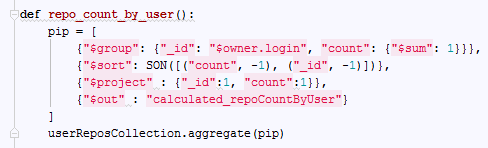
\includegraphics{Images/pymongo-aggregation.PNG}
%}
%\caption{Sample Python code which pulls the total repository count per user using PyMongo and the MongoDB Aggregation Framework.}
%\label{fig:repo-count-code}
%\end{center}
%\end{figure}


\subsection{Original vs. Forked Projects}
\label{origvsforked}
In order to determine original versus forked projects from our collection of local RTP projects, we needed to take a look at the "fork" field for each repository. The "fork" field takes a boolean value of True or False. We wrote a Python function that would count the number of original projects per user as well as the number of forked projects per user. Two separate collections were created in our local MongoDB instance and the data was later analyzed to help us understand if local users were forking existing projects more often than creating new projects.

\section{Overall RTP Activity}
Once we had established a baseline of GitHub users and associated repositories, we could start calculating RTP users' overall activity. As discussed, one piece of this research that particularly interested us was to find out how many users were actually active open source community members, in other words, how many users are actively contributing towards live projects. For this, we wanted to ignore users that joined for one project or homework assignment, for example, and never came back again. 

In order to gain an understanding of the overall GitHub activity in RTP, we investigated from a few different angles. We first aimed to understand trends in overall activity over the lifetime of a local user account and then wanted to understand who is still currently active. We are defining "active" in this research as making a commit to a repository over the last 6 months. In order to determine overall activity, we created the following questions to guide us:

\begin{enumerate}
\item Total number of commits by owner
\item Total number of active repositories based off commits
\item Total number of forks
\item Total number of pull requests
\item Total number of stargazers
\end{enumerate}

Question 1-2 are covered in section \ref{sec-commits}. Question 3 was covered already in section \ref{origvsforked}. Question 4 is covered in section \ref{sec-pullreqs} and question 5 is in section \ref{sec-stargazing}. The results from each data collection method are captured in Chapter \ref{Chapter:Findings}.

\subsection{Collecting User Commits and Active Repositories}
\label{sec-commits}
As part of the study of overall activity within our local scope, we sought to understand what the total number of commits per project looked like. In order to collect this information, we used the meta-data located in the GHTorrent MySQL instance in combination with our already existing collection of local users in our local MongoDB instance. We queried the GHTorrent MySQL instance for the name of the repository, the owner name, the count of commits as well as the last commit date. Figure~\ref{fig:commits-per-project} shows the script in detail. Due to the massive volume of commit data, we let this script run overnight as it took several hours to complete. During the initial run, we ran into errors that were not caught in the code. MongoDB requires UTF-8 encoding and hence any entries which were not UTF-8 that we tried to insert into our local MongoDB instance failed (\textbf{Error Message: bson.errors.InvalidStringData: strings in documents must be valid UTF-8}). We altered the script to translate these field names to binary to get past this, logging any future failure details to a new collection. The subsequent run of this script did not give us any failures, however. The total number of commits per project (as well as their associated timestamps) were useful is helping us answer defined questions on RTP user activity and current participation in the open source community.

\begin{figure}
\footnotesize
\begin{lstlisting}
def commit_numbers():

    query = "select p.name, u.login, u.name,
    max(c.created_at), count(c.id) 
    from projects p, users u, commits c"\
    " where u.id = p.owner_id"\
    " and c.project_id = p.id"\
    " and u.login = %s"\
    " and p.name = %s"\
    " group by p.name, u.login, u.name"

    reposList = userReposCollection.find(
    	{},{"owner.login":1, "name":1}) 
        
    i = 0
    try:
        for x in reposList:
            if(i > 16969):
                mySqlCursor = mySqlDB.cursor()
                mySqlCursor.execute(query,(x['owner']['login'],x['name']))
                data = mySqlCursor.fetchall()
                for row in data:
                    myLocalDB.testCollection.insert([
                        {"project_name":row[0],
                        "owner_login": row[1],
                        "owner_name": bson.Binary(str(row[2])),
                        "last_commit_date": row[3],
                        "commit_count":row[4]}])
                    print "done with ", x['owner']['login'], x['name'], i
            i+=1
            # print x['owner']['login'], x['name']
    except Exception, e:
        myLocalDB.rejects.insert({"failed":i})
\end{lstlisting}
\caption{This Python script was used to collect the number of commits per local project.}
\label{fig:commits-per-project}
\end{figure}

%\begin{figure}
%\begin{center}
%\resizebox{\textwidth}{!}{
%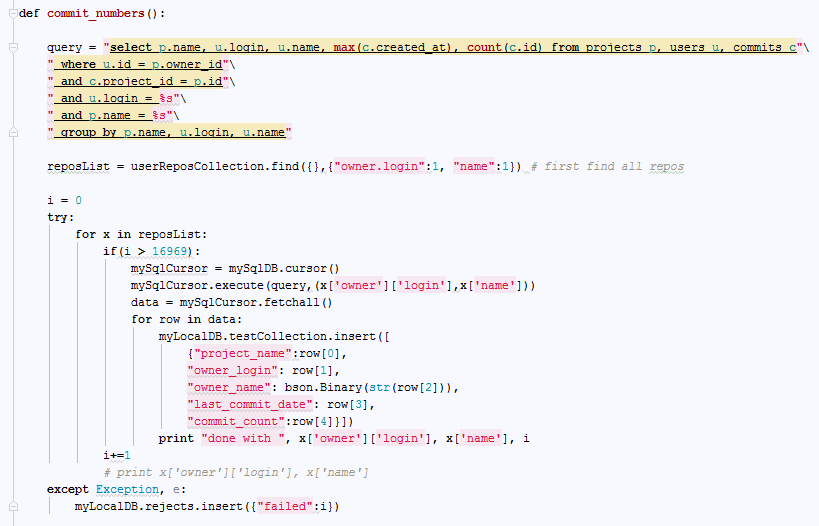
\includegraphics{Images/commitNumbers.PNG}
%}
%\caption{This Python script was used to collect the number of commits per local project.}
%\label{fig:commits-per-project}
%\end{center}
%\end{figure}

\subsection{Collecting Pull Requests}
\label{sec-pullreqs}
In order to determine overall user activity, we needed to understand how many pull requests had been submitted by each RTP user. For this, we pulled data directly out of the GHTorrent MySQL database and inserted it into our local MongoDB instance. The SQL query we used performed a union of two select statements. The first statement joins locally owned repositories on the head repository ID in the pull requests table and the second statement joins on the base repository id in the pull requests table. This is done to ensure we collect any repositories that have been forked. The script used for collecting the pull requests is shown in Figure \ref{fig:pullrequests}. 

\begin{figure}
\footnotesize
\begin{lstlisting}
def getPullReqs():

    query = "(select u.login, p.name, count(*) 
    	as 'prcount', 'head' as 'repotype'"\
            " from projects p, users u, pull_requests pr"\
            " where p.owner_id = u.id"\
            " and pr.head_repo_id = p.id"\
            " and p.deleted is false"\
            " and p.forked_from is null"\
            " and u.login = %s"\
            " group by p.id"\
            " order by count(*) desc)"\
            " UNION"\
            " (select u.login, p.name, count(*) 
            	as 'prcount', 'base' as 'repotype'"\
            " from projects p, users u, pull_requests pr"\
            " where p.owner_id = u.id"\
            " and pr.base_repo_id = p.id"\
            " and p.deleted is false"\
            " and p.forked_from is null"\
            " and u.login = %s"\
            " group by p.id"\
            " order by count(*) desc)"

    myUsers = githubRTPUsers.find({},{"login":1}) # first find all usernames

    i = 0
    try:
        for x in myUsers:
            mySqlCursor = mySqlDB.cursor()
            mySqlCursor.execute(query,(x['login'],x['login']))
            data = mySqlCursor.fetchall()
            for row in data:
                myLocalDB.calculated_pullReqByUser.insert([
                    {"login":row[0],
                    "name": row[1],
                    "prcount": row[2],
                    "repotype": row[3]}])
                print "done with ", x['login'], i
            i+=1
    except Exception, e:
        print e
        myLocalDB.rejects.insert({"failed":i})
\end{lstlisting}
\caption{Python script used to query for pull requests from the GHTorrent MySQL database and then insert them into our local MongoDB instance.}
\label{fig:pullrequests}
\end{figure}

\section{Social Networking - "Stargazing"}
\label{sec-stargazing}
In addition to overall open source activity, we were interested in understanding the popularity of local users and their work. One way to do this was to look into how many users had repositories which were being "starred" or "followed". We wrote a Python script to query the GHTorrent MongoDB instance (watchers collection), using our collected list of RTP users and their owned repositories. We inserted the results from this script into a new collection in our local MongoDB instance. Figure~\ref{fig:stargazers} shows an example of what one of these entries looks like. 

After the list of "stargazers" had been collected, we again used the MongoDB aggregation framework to find out which local repositories were the most popular.  Figure~\ref{fig:stargazers-count} shows what this query looked like. One thing to note for this collection is that if a user is a “contributor” on a project then the stars for that project end up in our list - some examples of this are shown in Chapter~\ref{Chapter:Findings} (Data Findings). Lastly, we utilized aggregation to find out how many followers each local user had (see Figure~\ref{fig:stargazing-aggregation}).

\begin{figure}
\tiny
\begin{lstlisting}
> db.githubRTPStargazers.findOne()
{
        "_id" : ObjectId("539eb518bd35432a2004564c"),
        "following_url" : "https://api.github.com/users/HagamosVideojuegos/following{/other_user}",
        "events_url" : "https://api.github.com/users/HagamosVideojuegos/events{/privacy}",
        "organizations_url" : "https://api.github.com/users/HagamosVideojuegos/orgs",
        "url" : "https://api.github.com/users/HagamosVideojuegos",
        "gists_url" : "https://api.github.com/users/HagamosVideojuegos/gists{/gist_id}",
        "html_url" : "https://github.com/HagamosVideojuegos",
        "subscriptions_url" : "https://api.github.com/users/HagamosVideojuegos/subscriptions",
        "repo" : "BombaFiesta-Unity3D-Futile",
        "owner" : "edbartley",
        "avatar_url" : "https://avatars.githubusercontent.com/u/6969130?",
        "repos_url" : "https://api.github.com/users/HagamosVideojuegos/repos",
        "received_events_url" : "https://api.github.com/users/HagamosVideojuegos/received_events",
        "gravatar_id" : "028308b2ed248bbd76fa686f0855006e",
        "starred_url" : "https://api.github.com/users/HagamosVideojuegos/starred{/owner}{/repo}",
        "site_admin" : false,
        "login" : "HagamosVideojuegos",
        "type" : "User",
        "id" : 6969130,
        "followers_url" : "https://api.github.com/users/HagamosVideojuegos/followers"
}
\end{lstlisting}
\caption{A view into the stargazers collection.}
\label{fig:stargazers}
\end{figure}

%\begin{figure}
%\begin{center}
%\resizebox{\textwidth}{!}{
%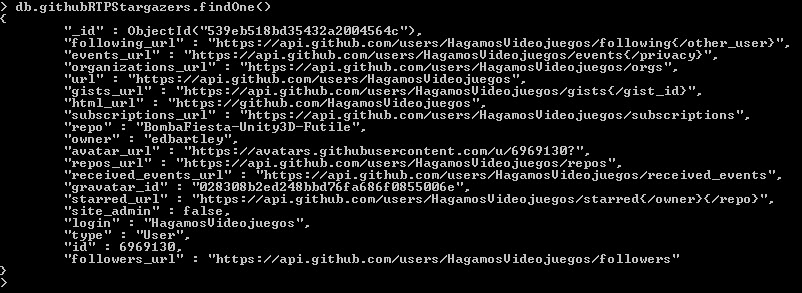
\includegraphics{Images/RTPStargazers_findOne.jpg}
%}
%\caption{A view into the stargazers collection.} 
%\label{fig:stargazers}
%\end{center}
%\end{figure}

\begin{figure}
\begin{lstlisting}
db.githubRTPStargazers.aggregate(
[
	{$group: {
    	_id:"$repo", 
        total: {$sum: 1}}},{$sort:{total:-1}
   	}
])
\end{lstlisting}
\caption{Aggregation used to find out how many followers each local repository contained.}
\label{fig:stargazers-count}
\end{figure}

\begin{figure}
\begin{lstlisting}
def stargazing():
    pip = [
        {"$group": {"_id": "$owner", "count": {"$sum": 1}}},
        {"$sort": SON([("count", -1), ("_id", -1)])},
        {"$project" : {"_id":1, "count":1, "owner":1,"repo":1}},
        {"$out" : "calculated_totalStargazers"}
    ]
    stargazersCollection.aggregate(pip)
\end{lstlisting}
\caption{Python script used to calculate the number of followers that each RTP user has.}
\label{fig:stargazing-aggregation}
\end{figure}

%\begin{figure}
%\begin{center}
%\resizebox{\textwidth}{!}{
%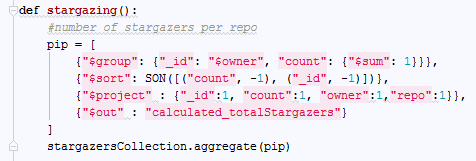
\includegraphics{Images/Stargazing-Aggregation.PNG}
%}
%\caption{Python script used to calculate the number of followers that each RTP user has.\label{fig:stargazing-aggregation}} 
%\end{center}
%\end{figure}
